% Terminal Basics - cover important commands such as sudo, apt-get etc.
In chapter \ref{chap:unity}  you have read about Ubuntu's graphical user interface (GUI), Unity. You have also seen how to install/uninstall new software, update software repositories and upgrade the system. The latter is is connected with chapter \ref{chap:software_management} because some of them will be shown here too. Basically, you are shown two ways to perform the same task. Which method you chose depends on what you like best. \\

\par \noindent In a terminal you can do anything and everything than can done through a GUI. It varies from the most bast tasks such as  creating/removing directories and files, moving/copying  directories and files to advanced things like configuring your local area network (LAN), send mails and connect to remote server. \\

\par \noindent In this manual only the basics will be shown. Before you go any further please open a terminal. To open the terminal, click  on the Dash button and just search for terminal as shown in figure \ref{fig:open-terminal}. 

\begin{figure}[h]	
	\centering
	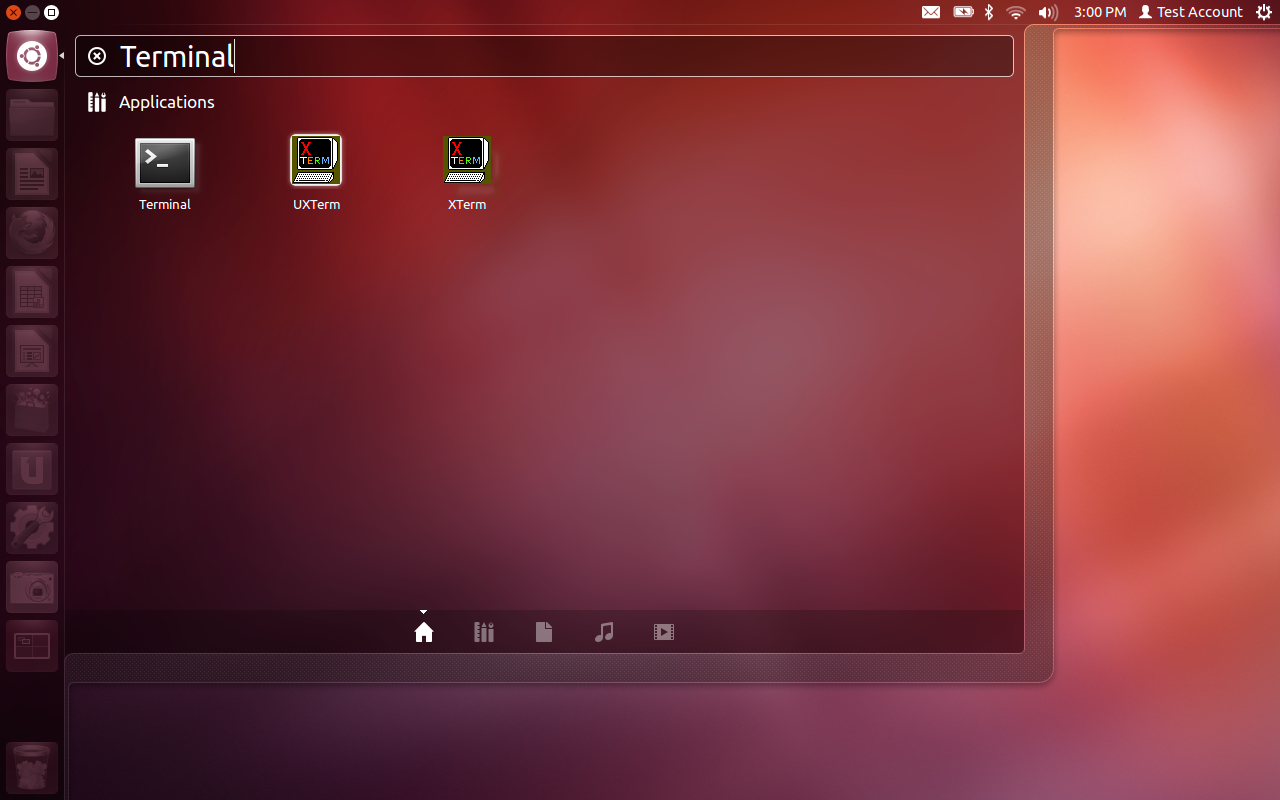
\includegraphics[width=400pt]{./images/terminal/open-terminal.png}
	\caption{Open terminal using dash}	
	\label{fig:open-terminal}	
\end{figure}

\par \noindent After that, you just left click on a terminal and wait for it to open. If you have done everything right, you should see the terminal window as shown in figure \ref{fig:terminal-window}.  \\

\begin{figure}[h]	
	\centering
	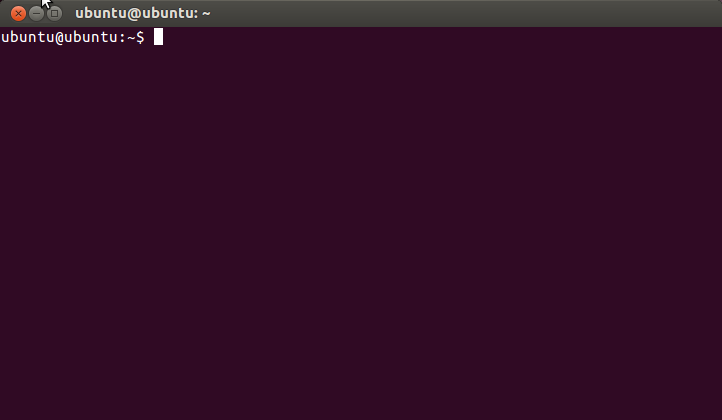
\includegraphics[width=300pt]{./images/terminal/terminal-window.png}
	\caption{Terminal Window}	
	\label{fig:terminal-window}	
\end{figure}

\par \noindent \framebox[6.7in][l]{\parbox[l]{6.5in}{\textbf{Note}: Examples from this point forward are  done in Ubuntu Lucid Lynx 10.04. Reason for that is due to Precise Pangolin being a test version while this tutorial is written.  (You will have Precise Pangolin labels if you installed it). Everything is same considering terminal and commands though. Prior pictures are taken under USB live running Precise Pangolin.}} \\ \\

\par \noindent With the terminal open, you can see a line of text.  What does this line of text indicate? First part of the text is your username. Also it states your /home partition. Second part of the text is your computer's name. This text also indicates which directory you are currently on. You can also check the current directory you are in by executing the \textit{pwd} command. For example,if the text is similar as shown in figure \ref{fig:pwd-command}, it means that you are now at home, to be more precise /home partition. \\

\begin{figure}[h]	
	\centering
	\fbox{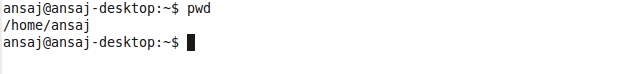
\includegraphics[width=350pt]{./images/terminal/pwd-command.png}}
	\caption{pwd command}	
	\label{fig:pwd-command}	
\end{figure}

\par \noindent You can check that you are in a /home partition by just typing \textit{ls} command and pressing Enter. If you have done everything right you should see all files and folders that are under your /home partition. That is your data. See figure \ref{fig:ls-command} \\

\begin{figure}[h]	
	\centering
	\fbox{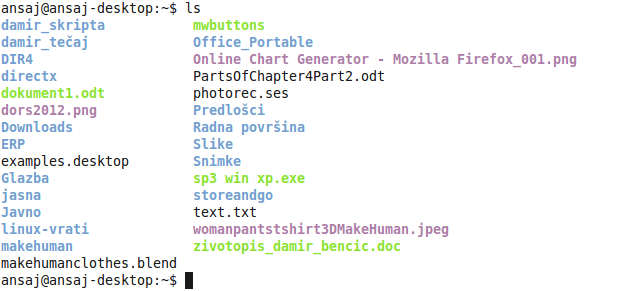
\includegraphics[width=350pt]{./images/terminal/ls-command.png}}
	\caption{ls command}	
	\label{fig:ls-command}	
\end{figure}

\par \noindent The command \textit{ls} lists all the files and folders in the directory you are currently on. Once the files and folders are shown, the terminal is waiting for you to type another command. This was basically just a small introduction to the terminal basics. Before learning about other commands, it is first essential to know about the different type of users to better understand the need for the commands covered later. \\

\par \noindent In chapter \ref{chap:about_ubuntu_why},  you read about Ubuntu's multi-user environment feature. You can be either an administrator or just a standard user. As an administrator you have more privileges than a standard user. On install by default you are provided with an administrator account meaning you have all the privileges unlike other people to whom you give  your computer for usage. \\

\par \noindent Let's proceed to the more important commands that are worth mentioning.

\section{SUDO command} \index{Sudo} \index{Terminal!Sudo}
% SUDO command - Describe
Commands such as \textit{ls}, are commands that every user can execute. In this chapter, commands that only the administrator of a computer can execute will be shown. \\

\par \noindent Sudo stands for  super user do (something that only an administrator can execute or do). This is not a command by itself but is rather used in combination with other commands that require administrative privileges. By using the sudo command, you are instructing the computer to run a command as an administrator. For example, let's try to update the system without sudo command. Type \textit{apt-get update} in the terminal and press Enter. After you have done that you should see something like shown in figure \ref{fig:sudo1}. \\

\begin{figure}[h!]	
	\centering
	\fbox{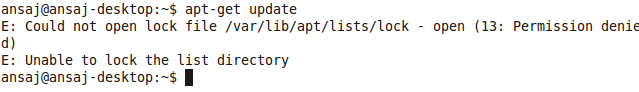
\includegraphics[width=350pt]{./images/terminal/sudo1.png}}
	\caption{apt-get update without sudo command}	
	\label{fig:sudo1}	
\end{figure}

\par \noindent If you got an error, that is a good sign. This just shows you that you cannot execute command apt-get update without the  sudo command in front of it. What the system does is to try to update the system as a regular user. Now, repeat the former step again but now type sudo in front of it  \textit{sudo apt-get update} and press Enter. You should be prompted with the administrator's password request. Type your password and press enter.  See figure \ref{fig:sudo2}.\\

\begin{figure}[h!]	
	\centering
	\fbox{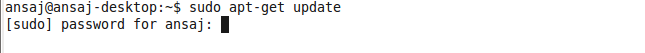
\includegraphics[width=350pt]{./images/terminal/sudo2.png}}
	\caption{sudo apt-get update}	
	\label{fig:sudo2}	
\end{figure}

\par \noindent Do not worry if you don't see what you are typing. It is invisible but you are typing it though (invisibility is for security reasons). After you have finished just press Enter. You should see something like shown in figure \ref{fig:sudo3}. (The computer is updating its database of the latest software available for your computer.). \\

\begin{figure}[h!]	
	\centering
	\fbox{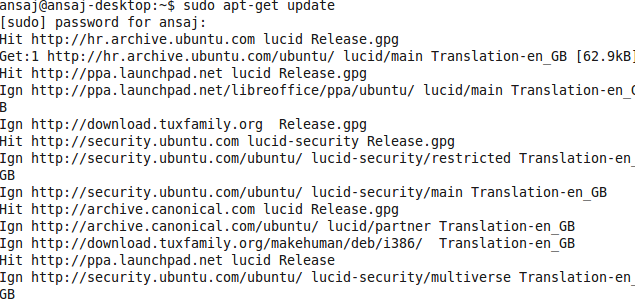
\includegraphics[width=350pt]{./images/terminal/sudo3.png}}
	\caption{Updating system's software database}	
	\label{fig:sudo3}	
\end{figure}

\par \noindent By now you should understand how the sudo command works. Later on there will be more examples showing the usage of the sudo command. \\

\par \noindent Note: Once you have entered  your password after sudo [-command-], the administrative mode is available for few minutes. This means that you can run other sudo [-command-] without entering the password. This mode becomes unavailable after a few minutes or after you close the terminal. \\

\section{Creating/Removing directories and files} \index{Terminal!Create/Remove} 
You probably know how to create folder or directory and file through the GUI. Here you will do those things via a terminal. The command to create a directory is mkdir. \\

\par \noindent \framebox[6.7in][l]{\parbox[l]{6.5in}{\textbf{Note}: If you give your directory a name via the terminal that has two or more words namely My pictures, you will have to connect those words with an underscore (\_). If you don't connect them with an underscore then the command will create two directories called My and pictures.}} \\

\par \noindent  Enter the command mkdir to create a folder in the terminal. This is illustrated in figure \ref{fig:mkdir1}.

\begin{figure}[h!]	
	\centering
	\fbox{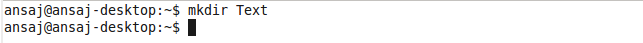
\includegraphics[width=350pt]{./images/terminal/mkdir1.png}}
	\caption{Create a new directory}	
	\label{fig:mkdir1}	
\end{figure}

\par \noindent If nothing happens and you are prompted with your address again then everything is all right. To check that you have created folder type ls command and scroll down a bit to see if it is there. 

\begin{figure}[h!]	
	\centering
	\fbox{
\includegraphics[width=350pt]{./images/terminal/mkdir2.png}}
	\caption{Directory Text}	
	\label{fig:mkdir2}	
\end{figure}
 
\par \noindent You can also check it via the graphical user interface. Go to the home directory to see if it is there. Suddenly you have decided that  you don't need that directory anymore. You can delete it. But let's try to do this using the terminal. Open your terminal again and type \textit{sudo rmdir Text}. Command rmdir is used to remove files and directories.

\begin{figure}[h!]	
	\centering
	\fbox{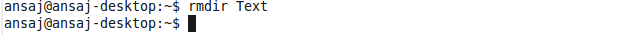
\includegraphics[width=350pt]{./images/terminal/rmdir1.png}}
	\caption{Remove directory}	
	\label{fig:rmdir1}	
\end{figure}

\par \noindent You can check if you have removed it from home folder/partition like explained before ( either ls or the GUI). As a small exercise, create another directory named Text. You will put files that you will create shortly after this into this folder. Now, type the command \textit{cd Text} and press Enter.  Command \textit{cd} lets you to navigate directories. In this case, you navigated into the Text directory. If you have done the cd command right, you should see something as shown in  illustration \ref{fig:mkdir4}.\\

\begin{figure}[h!]	
	\centering
	\fbox{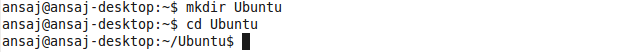
\includegraphics[width=350pt]{./images/terminal/mkdir4.png}}
	\caption{Create new directory called Ubuntu}	
	\label{fig:mkdir4}	
\end{figure}

\par \noindent To get out of the directory just type \textit{cd} and  press Enter and nothing else. You should be back to your home directory. Next is to learn how to create a file. You should already know how to create a file via some text editor like Word, Writer, notepad etc. Here you will also need an editor to create a file. Default editor that comes with terminal is called gedit. That tool is going to be used here for examples. \\

\par \noindent \framebox[6.7in][l]{\parbox[l]{6.5in}{\textbf{Note}: File names have the same rules as directory. If you have two or more words connect them with underscore (\_). Text files in gedit have .txt extension.}} \\

\par \noindent To create a file that will be automatically saved in some directory command should look like this: gedit  file\_name.txt. Navigate into the directory named Text you created before. Let's create a file named ubuntu\_releases.txt. type into the terminal as shown in the illustration... and press Enter. (gedit  ubuntu\_releases.txt) \\

\begin{figure}[h!]	
	\centering
	\fbox{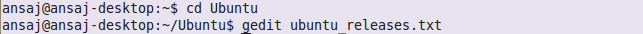
\includegraphics[width=350pt]{./images/terminal/mkdir5.png}}
	\caption{Create file}	
	\label{fig:mkdir5}	
\end{figure}

\par \noindent Soon you will be prompted with gedit editor, (perhaps you will be prompted with request for writing an administrators password). \\

\begin{figure}[h!]	
	\centering
	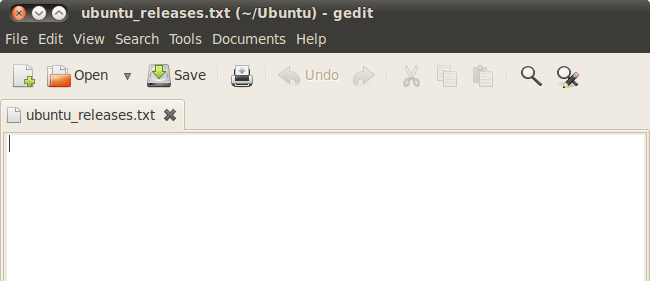
\includegraphics[width=350pt]{./images/terminal/mkdir6.png}
	\caption{Create file - Gedit Window}	
	\label{fig:gedit}	
\end{figure}

\par \noindent You can type into that editor just like any other. Also you can save what you have written. Try to type some of the Ubuntu releases namely: Lucid Lynx, Precise Pangolin etc. To save just do what you used to do in other editors by pressing CTRL+S. After you are done close the editor by clicking on the x sign in the upper left corner.  \\

\par \noindent \framebox[6.7in][l]{\parbox[l]{6.5in}{\textbf{Note}:  The text file will be saved in the directory from where you started the gedit editor. If you where in Ubuntu directory as shown in illustration \ref{fig:mkdir5}, then you should find your file named ubuntu\_releases.txt under that directory.  Later on it will be shown how to move and copy a file from one directory to other. }} \\

\par \noindent Before proceeding to copying and moving files lets first learn how to delete a file. Open your terminal if it is closed and check where your ubuntu\_releases.txt file. Hint (\textit{ls} to list what files and folders  you have in some directory, then cd  $<directory\_name>$ to enter and exit some directory.  \\

\par \noindent Deleting a file is similar process like deleting a folder or a directory. The only difference is the command. For deleting a file you have to write: \textit{rm file\_name} and press Enter. If you found your file (if you followed this tutorial it should be in your home folder. Type rm ubuntu\_releases.txt and press enter. To convince yourself that you deleted a file type ls or through the file manager. 

\begin{figure}[h!]	
	\centering
	\fbox{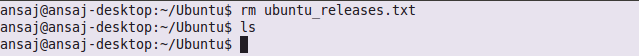
\includegraphics[width=350pt]{./images/terminal/rm1.png}}
	\caption{Delete file}	
	\label{fig:rm1}	
\end{figure}

\section{Moving/Copying directories and files} \index{Terminal!Move/Copy}
In this section you will see how to copy directory/file, move directory/file and remove the entire directory with all files at once. \\

\par \noindent To copy a directory  you should use this syntax, \fbox{cp  -r  directory\_name1 directory\_name2} where, \\

\par \noindent directory\_name1: Directory that you want to copy \\
directory\_name2: Directory where you want to copy directory\_name1 \\
-r :  this flag enables you to copy entire directory. The cp command alone copies only files. \\

\par \noindent As an exercise, let's create a new directory and name it DIR1 (hint:  \textit{mkdir DIR1}). After that create another directory and name it DIR2. Now try to copy DIR1 into DIR2 by executing \textit{cp -r DIR1 DIR2}. If everything went all right, you should find copy of a DIR1 under DIR2 as shown in figure \ref{fig:cp1}. \\

\begin{figure}[h!]	
	\centering
	\fbox{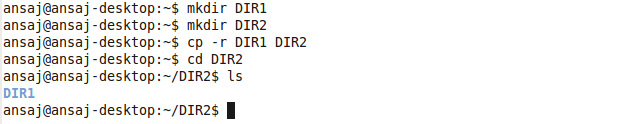
\includegraphics[width=350pt]{./images/terminal/cp1.png}}
	\caption{Copy directory}	
	\label{fig:cp1}	
\end{figure}

\par \noindent \framebox[6.7in][l]{\parbox[l]{6.5in}{\textbf{Note}: Notice that in the examples above you were working in your home folder. When you will want to copy folders/files in some other destinations you will have to use slash  / . With slash you tell the path where you want to copy something. For example you create another directory under DIR2 named DIR3. You decide that you want to copy some files from home folder to DIR3. It would go like this: \textit{cp  file\_name  DIR2/DIR3}  + enter. }} \\

\par \noindent Sometimes too many copies of something is not good. You would like to instead move them. So for moving or cutting a directory or a file the command mv is used. The command mv can also be used to rename files and directories. You should use the following syntax, \\

\par \noindent \fbox{mv directory\_name1  directory\_name2} \\

\par \noindent directory\_name1: folder you want to move or cut \\
directory2\_name: destination folder \\

\par \noindent Try to move already created and copied DIR1 into DIR2.  To do that execute \textit{sudo mv DIR1 DIR2} and hit Enter. If everything went all right you should have only one DIR1 under DIR2 and nowhere else. Check that with already mentioned command \textit{ls}. See figure \ref{fig:mv1}.

\begin{figure}[h!]	
	\centering
	\fbox{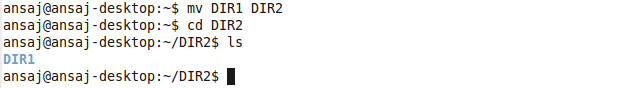
\includegraphics[width=350pt]{./images/terminal/mv1.png}}
	\caption{Move directory}	
	\label{fig:mv1}	
\end{figure}

\par \noindent How do you copy or move a file? It is similar to copying or moving directories. The same commands cp and mv are used. However the syntax is slightly different. To copy a file the syntax is \fbox{sudo cp file name destination}. Create a new file named file1.txt (hint:  \textit{sudo gedit file1.txt}, save it and exit from gedit). To copy it into DIR2 execute \textit{sudo  cp  file1.txt  DIR2} and hit Enter. (Check if file is copied with commands cd and ls). See figure \ref{fig:cp2}.

\begin{figure}[h!]	
	\centering
	\fbox{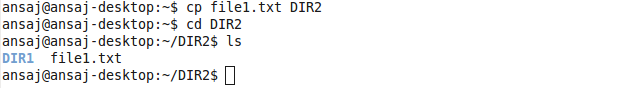
\includegraphics[width=350pt]{./images/terminal/cp2.png}}
	\caption{Copy file}	
	\label{fig:cp2}	
\end{figure}

\par \noindent To move a file the syntax is \fbox{sudo mv file name destination}. The procedure is similar to copying. The only difference is the command. Execute \textit{sudo mv file1.txt DIR2} and press enter. \\

\par \noindent \framebox[6.7in][l]{\parbox[l]{6.5in}{\textbf{Note}: If you will be prompted with message that old file1.txt in DIR2 will be overwritten just type y and press enter. After that your file should be only under DIR2 directory. See figure \ref{fig:mv2}.}} \\

\begin{figure}[h!]	
	\centering
	\fbox{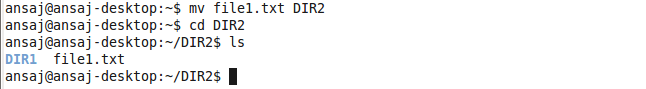
\includegraphics[width=350pt]{./images/terminal/mv2.png}}
	\caption{Move file}	
	\label{fig:mv2}	
\end{figure}

\par \noindent What if you decide that you don't need all these directories and files? Under GUI you would just delete it with one click. Here you will delete it with one command. How to delete one file and directory you know (hint: commands rm and rmdir). To remove directory and all its content syntax is \fbox{rm -R directory\_name}.  (-R flag helps you to remove entire directory together with its content) \\

\par \noindent Try removing DIR2 by typing: sudo rm -R DIR2 and press enter. If everything went alright, DIR2 doesn't exist in home folder anymore.  See figure \ref{fig:mv3}. To convince yourself, check via GUI or via ls in terminal.  \\

\begin{figure}[h!]	
	\centering
	\fbox{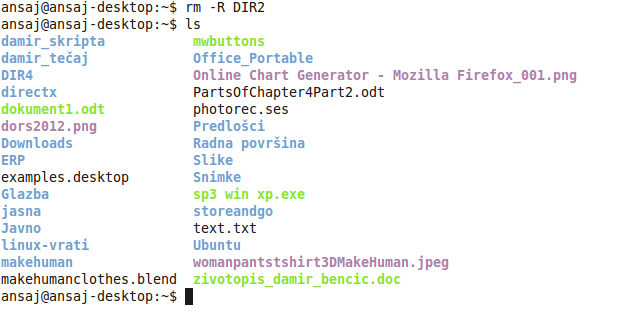
\includegraphics[width=350pt]{./images/terminal/mv3.png}}
	\caption{Remove directory with content}	
	\label{fig:mv3}	
\end{figure}

\section{Submitting bug reports} \label{sect:bugreport-terminal} \index{Bug} 
As described in section \ref{chap:about_ubuntu_contribute}, bug reports are managed in Launchpad. It is one central place where the Ubuntu developers manage the bug submitted by users and try to fix the issues. Submitting bug reports to Launchpad can be easily done via the terminal using one simple command. This is illustrated in this section. In order to submit bug reports, you need to know the name of the package you are reporting the bug against. Once you know the name of the package, type \fbox{ubuntu-bug package\_name} as shown in figure \ref{fig:bugreport1}

\begin{figure}[h!]	
	\centering
	\fbox{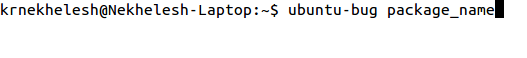
\includegraphics[width=350pt]{./images/terminal/bugreport1.png}}
	\caption{Submit bug report}	
	\label{fig:bugreport1}	
\end{figure}

\par \noindent When you execute this command in the terminal, Ubuntu will collect all necessary information about your system automatically and create a bug report in Launchpad. You are however required to enter a bug title, description on how to reproduce this and provide any screenshots if necessary. A well described bug report will help the developers identify the problem quickly and solve the issue. It will then be issued as an update to all the Ubuntu users. \\

\par \noindent Some common package names are mentioned here. If it is graphical issue the most probable package is \emph{compiz}. So then you would type \emph{ubuntu-bug compiz}. If the bug is related to the dash or launcher, the package name is \emph{unity}. If you are unable to find the package name, just use of the above mentioned package names. The bug triagers will relate it to the correct package for you.

\newpage
\section{Installing/Uninstalling packages} \index{Terminal!Update/Upgrade packages}
You have already  seen how to install/uninstall packages via the Ubuntu Software Center. This section will show how to do this using the terminal. The command used for everything related to packages is called apt-get. For installing/uninstalling/removing software to be possible via the terminal, every distribution including Ubuntu has a ``package system that uses a private package database to keep track of which packages are installed, which are not installed and which are available for installation on your system. Considering installation, the apt-get command uses this database to find out how to install packages requested by the user and to find out which additional packages are needed in order for a selected package to work properly." \\

\par \noindent This section will cover the following topics,

\begin{itemize}
	\item update software repositories (mentioned database)
	\item upgrade system with new packages
	\item install/uninstall applications
	\item remove packages that are not needed any more
\end{itemize}

\par \noindent These are basic things and it is good to know them. This is just a start. You have to be aware that not everything can be configured or installed via GUI. Eventually you will have to step into terminal. It is similar to a car. You eventually will have to open the hood and check for the engine and the rest of the parts. The terminal also provides a way to perform task quickly without much delay.\\

\par \noindent Updating the package database is important so you can install newer versions of a software.  Without updating the database you could find yourself with errors like: some packages could not be installed or reached, invalid address etc. First part, updating a system's database you need to execute \textit{sudo apt-get update},  please see illustrations 7.8. and 7.9. \\

\par \noindent For upgrading the system's database with new packages you have to execute the command \textit{sudo apt-get dist-upgrade}.  If you wrote command correctly you should see something like illustration (number required).  You will be also prompted with question do you want to install update packages (for yes press y+enter, and for no press n+enter) as can be in figure \ref{fig:dist-upgrade}. \\

\begin{figure}[h!]	
	\centering
	\fbox{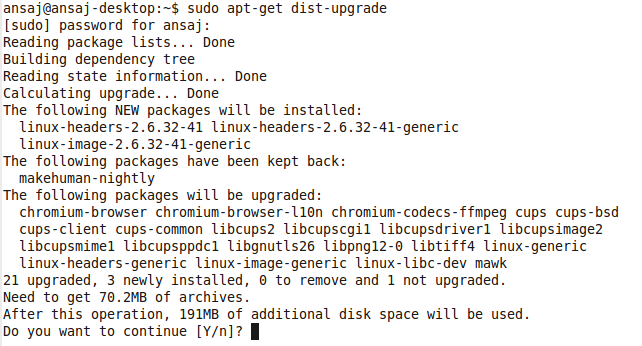
\includegraphics[width=350pt]{./images/terminal/dist-upgrade.png}}
	\caption{Upgrading system with new packages}	
	\label{fig:dist-upgrade}	
\end{figure}

\par \noindent Regular updating and upgrading your system's database helps you not just stay up-to-date as already mentioned but it helps your system to work properly. As you could have seen during an upgrade,  you didn't choose which packages to install, apt-get did it automatically for you. You just had to press y or n (yes or no). \\

\par \noindent You can also install package or a program individually by yourself. You saw how it is done via Ubuntu Software Center. With just one click you installed some applications. Here you will learn to install an application using just one command. You have to be careful that you don't fill your system with all kinds untrustworthy applications. That can cause you problems. Be careful what applications you install and from what source. It is recommended that you install what is in Ubuntu's database (better known repository). The easiest way to check that, is to visit Ubuntu's software center and type the name of an application. If it's not found there than you are installing an application at your own risk. \\

\par \noindent For installing an application  you have to execute \textit{sudo apt-get install $<application\_name>$ }\\

\par \noindent As simple as this is, you could hit a potential road block. You have to know what is the right name of a package or application so that you could install it. The Internet helps a lot in these situations. So don't worry. First is to try writing the application's name with lower case letters. For example if you don't have Skype installed on your system. Try executing \textit{sudo apt-get install skype}. If everything went all right you should see something like figure \ref{fig:install-skype}. \\

\begin{figure}[h!]	
	\centering
	\fbox{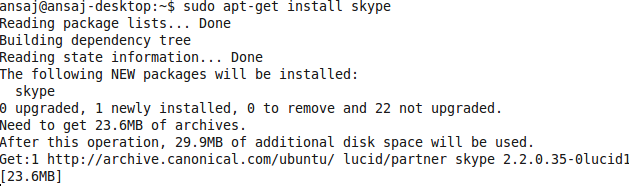
\includegraphics[width=350pt]{./images/terminal/install-skype.png}}
	\caption{Installing Skype}	
	\label{fig:install-skype}	
\end{figure}

\par \noindent After the installation is complete, you should see skype under your GUI (Ubuntu Software Center/Installed applications). 
If you decide to remove Skype, execute \textit{sudo apt-get remove skype} and press enter. The procedure is basically the same as with installation but is the other way around. Also, procedure is basically the same with other applications, \textit{ sudo apt-get remove <application\_name>} If you  typed command properly you should see something like figure \ref{fig:uninstall-skype}. \\

\begin{figure}[h!]	
	\centering
	\fbox{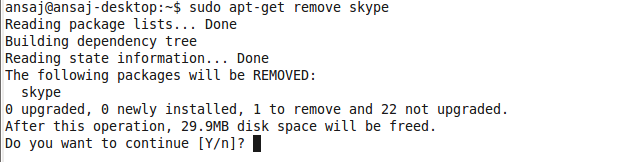
\includegraphics[width=350pt]{./images/terminal/uninstall-skype.png}}
	\caption{Uninstalling Skype}	
	\label{fig:uninstall-skype}	
\end{figure}

\par \noindent While using your system you might want to clean up unwanted packages left by some applications that are taking place on your disk. These packages were used by your system till one point. As the system is upgraded it doesn't need old ones, instead uses the new ones. So the old ones can be deleted. To remove unwanted/not needed packages execute \textit{sudo apt-get autoremove} and press enter. See figure \ref{fig:Autoremove}. \\

\begin{figure}[h!]	
	\centering
	\fbox{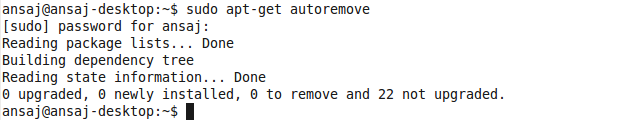
\includegraphics[width=350pt]{./images/terminal/autoremove.png}}
	\caption{Autoremove command}	
	\label{fig:Autoremove}	
\end{figure}

\par \noindent Tip: you can also use commands clean and autoclean.  \\

\par \noindent Do not think that this is it. There is much more. That ``much more" you will find at the Ubuntu official help pages. This will be described in more detail at the end of this manual. For conclusion of this chapter, Terminal is a very strong tool. Lot of ``stuff" can be fixed and configured here. You can see everything from different perspective and learn much more how system ``breathes". You don't have to memorise all commands. You have help/man. Use it wisely. 
